\documentclass[11pt]{article}
\usepackage[margin=1in]{geometry}
\usepackage{graphicx}
\usepackage{booktabs}
\usepackage{float}

\title{ELEC5660 Project 1 Phase 1 Report}
\author{SIT, IOK LONG}
\date{\today}

\begin{document}
\maketitle

\section{Introduction}

I have completed the controller by following lecture notes3 page 46. Additionally, added two trajectory called diamond and heart.

\section{experiment}

\begin{figure}[H]
\centering
\begin{minipage}{0.32\linewidth}
\centering
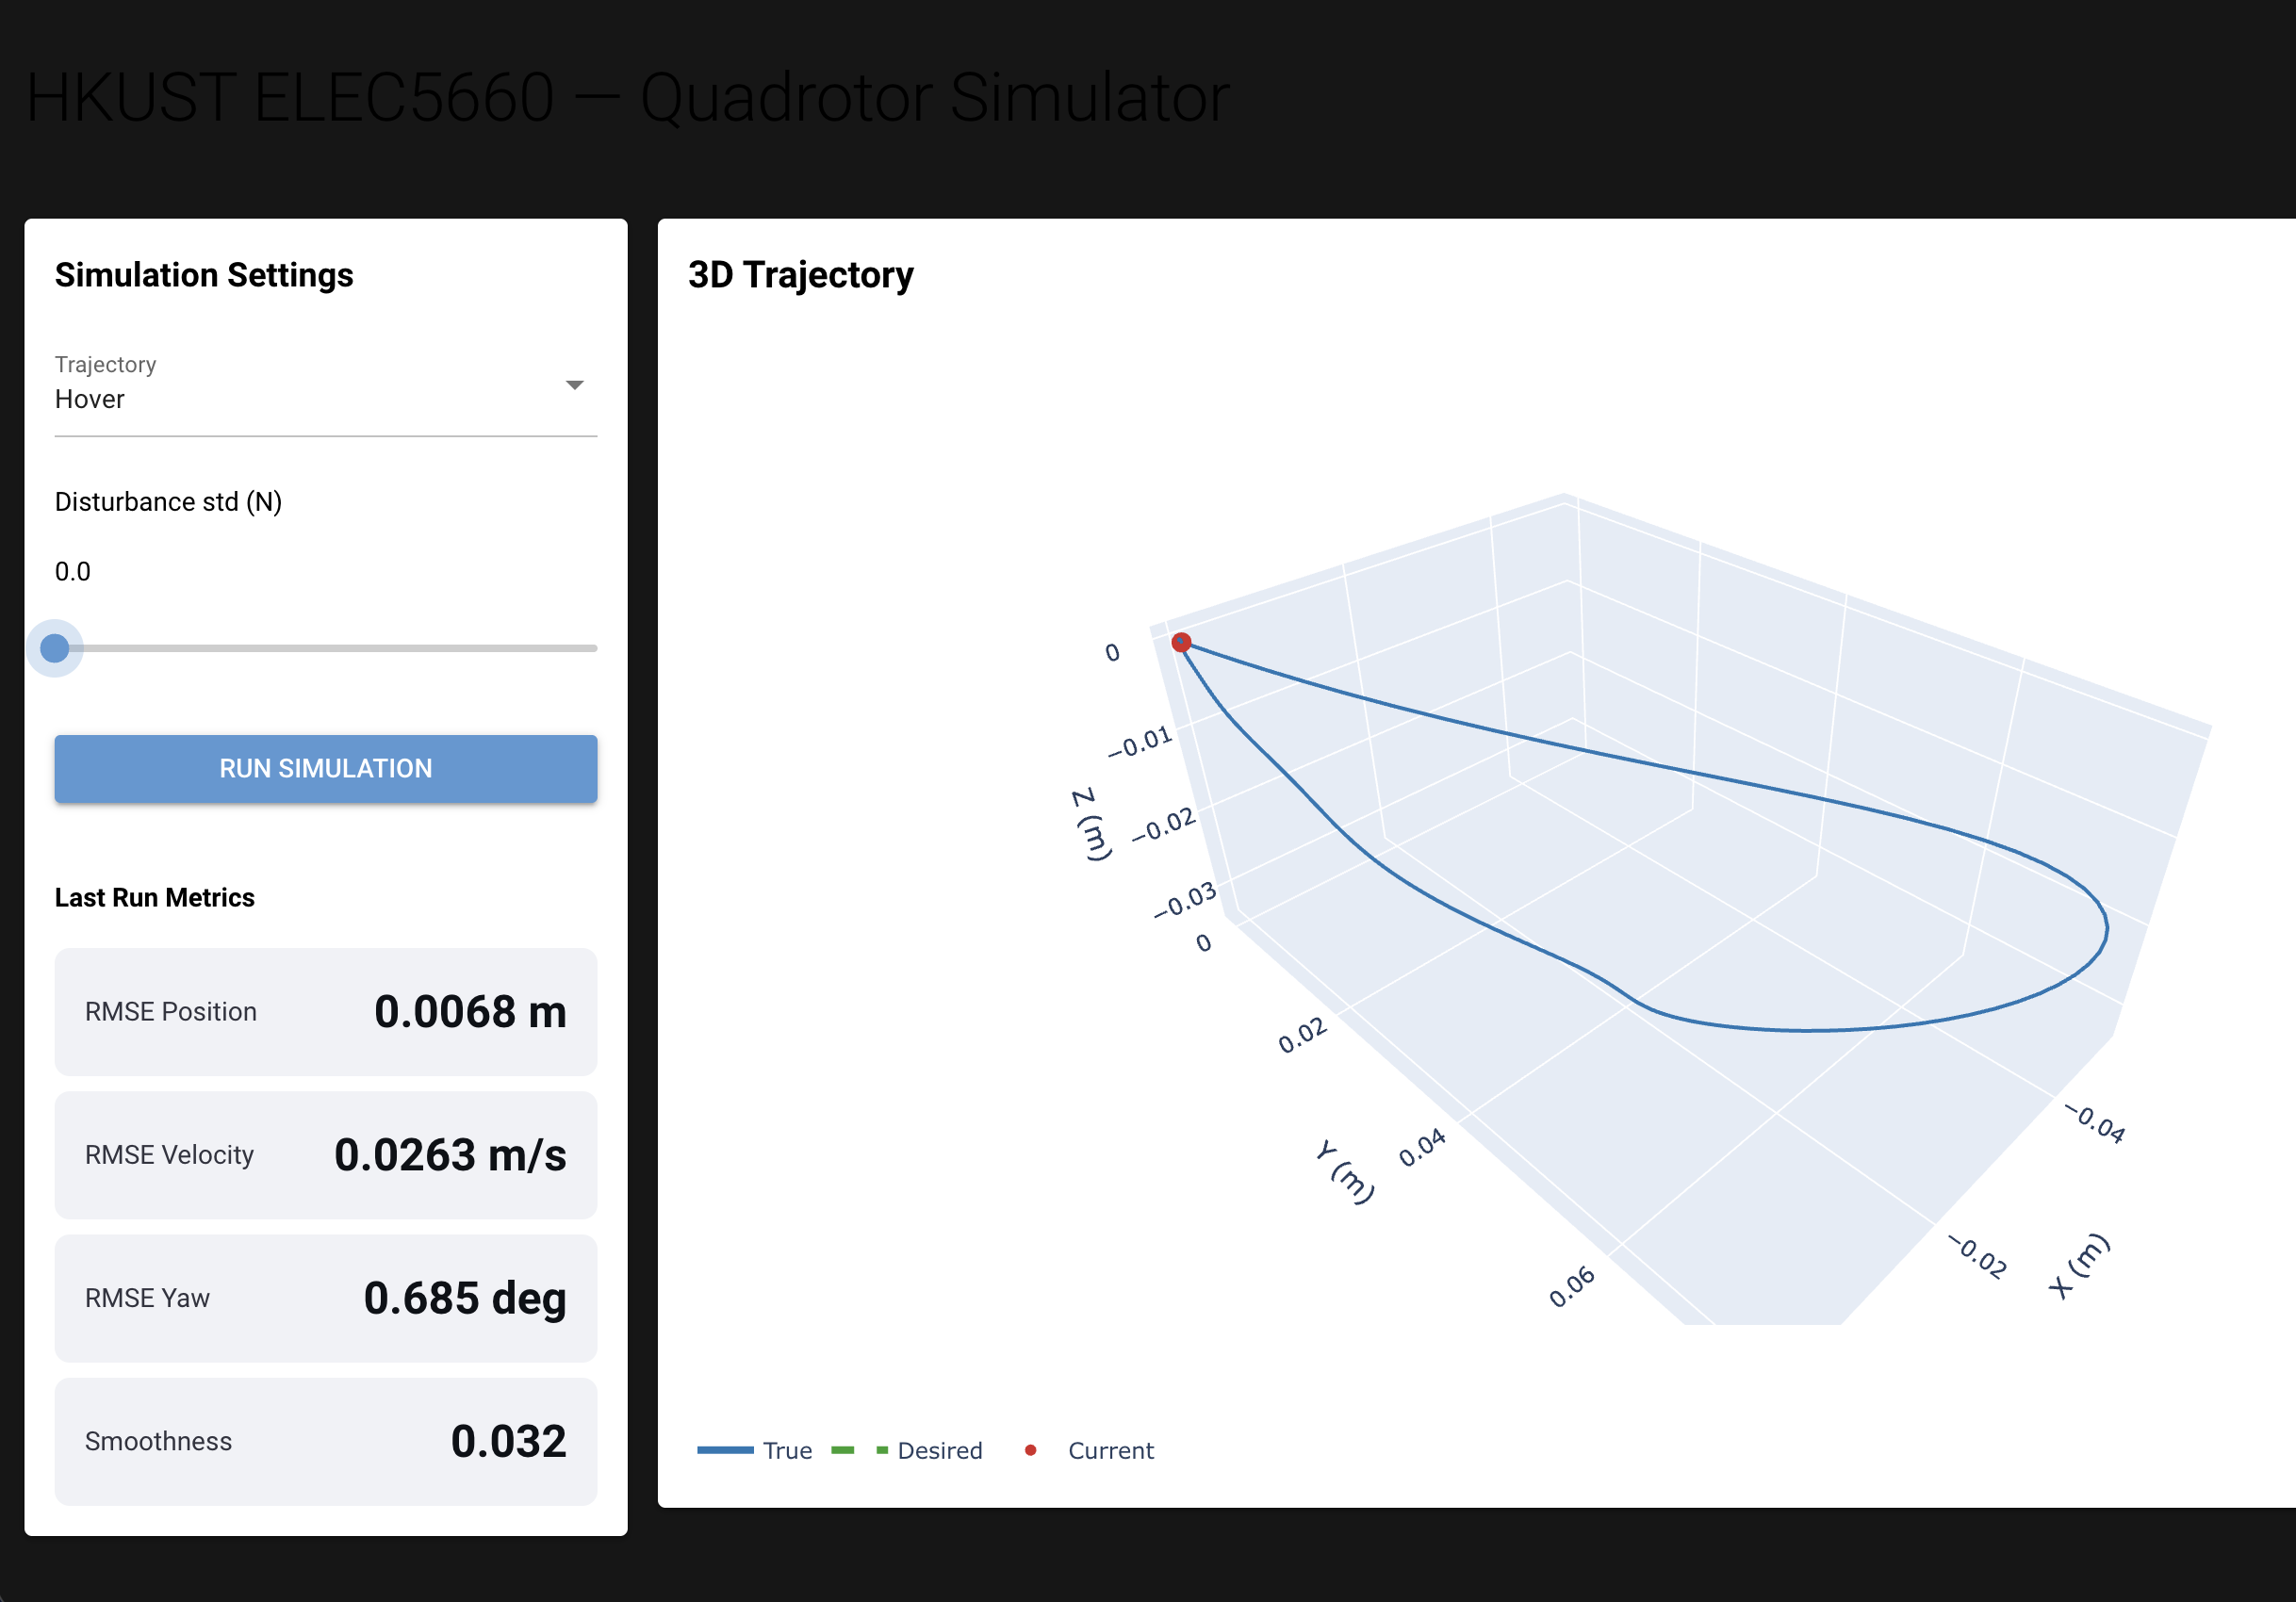
\includegraphics[width=\linewidth]{figs/1.png}
\caption*{hover}
\end{minipage}
\hfill
\begin{minipage}{0.32\linewidth}
\centering
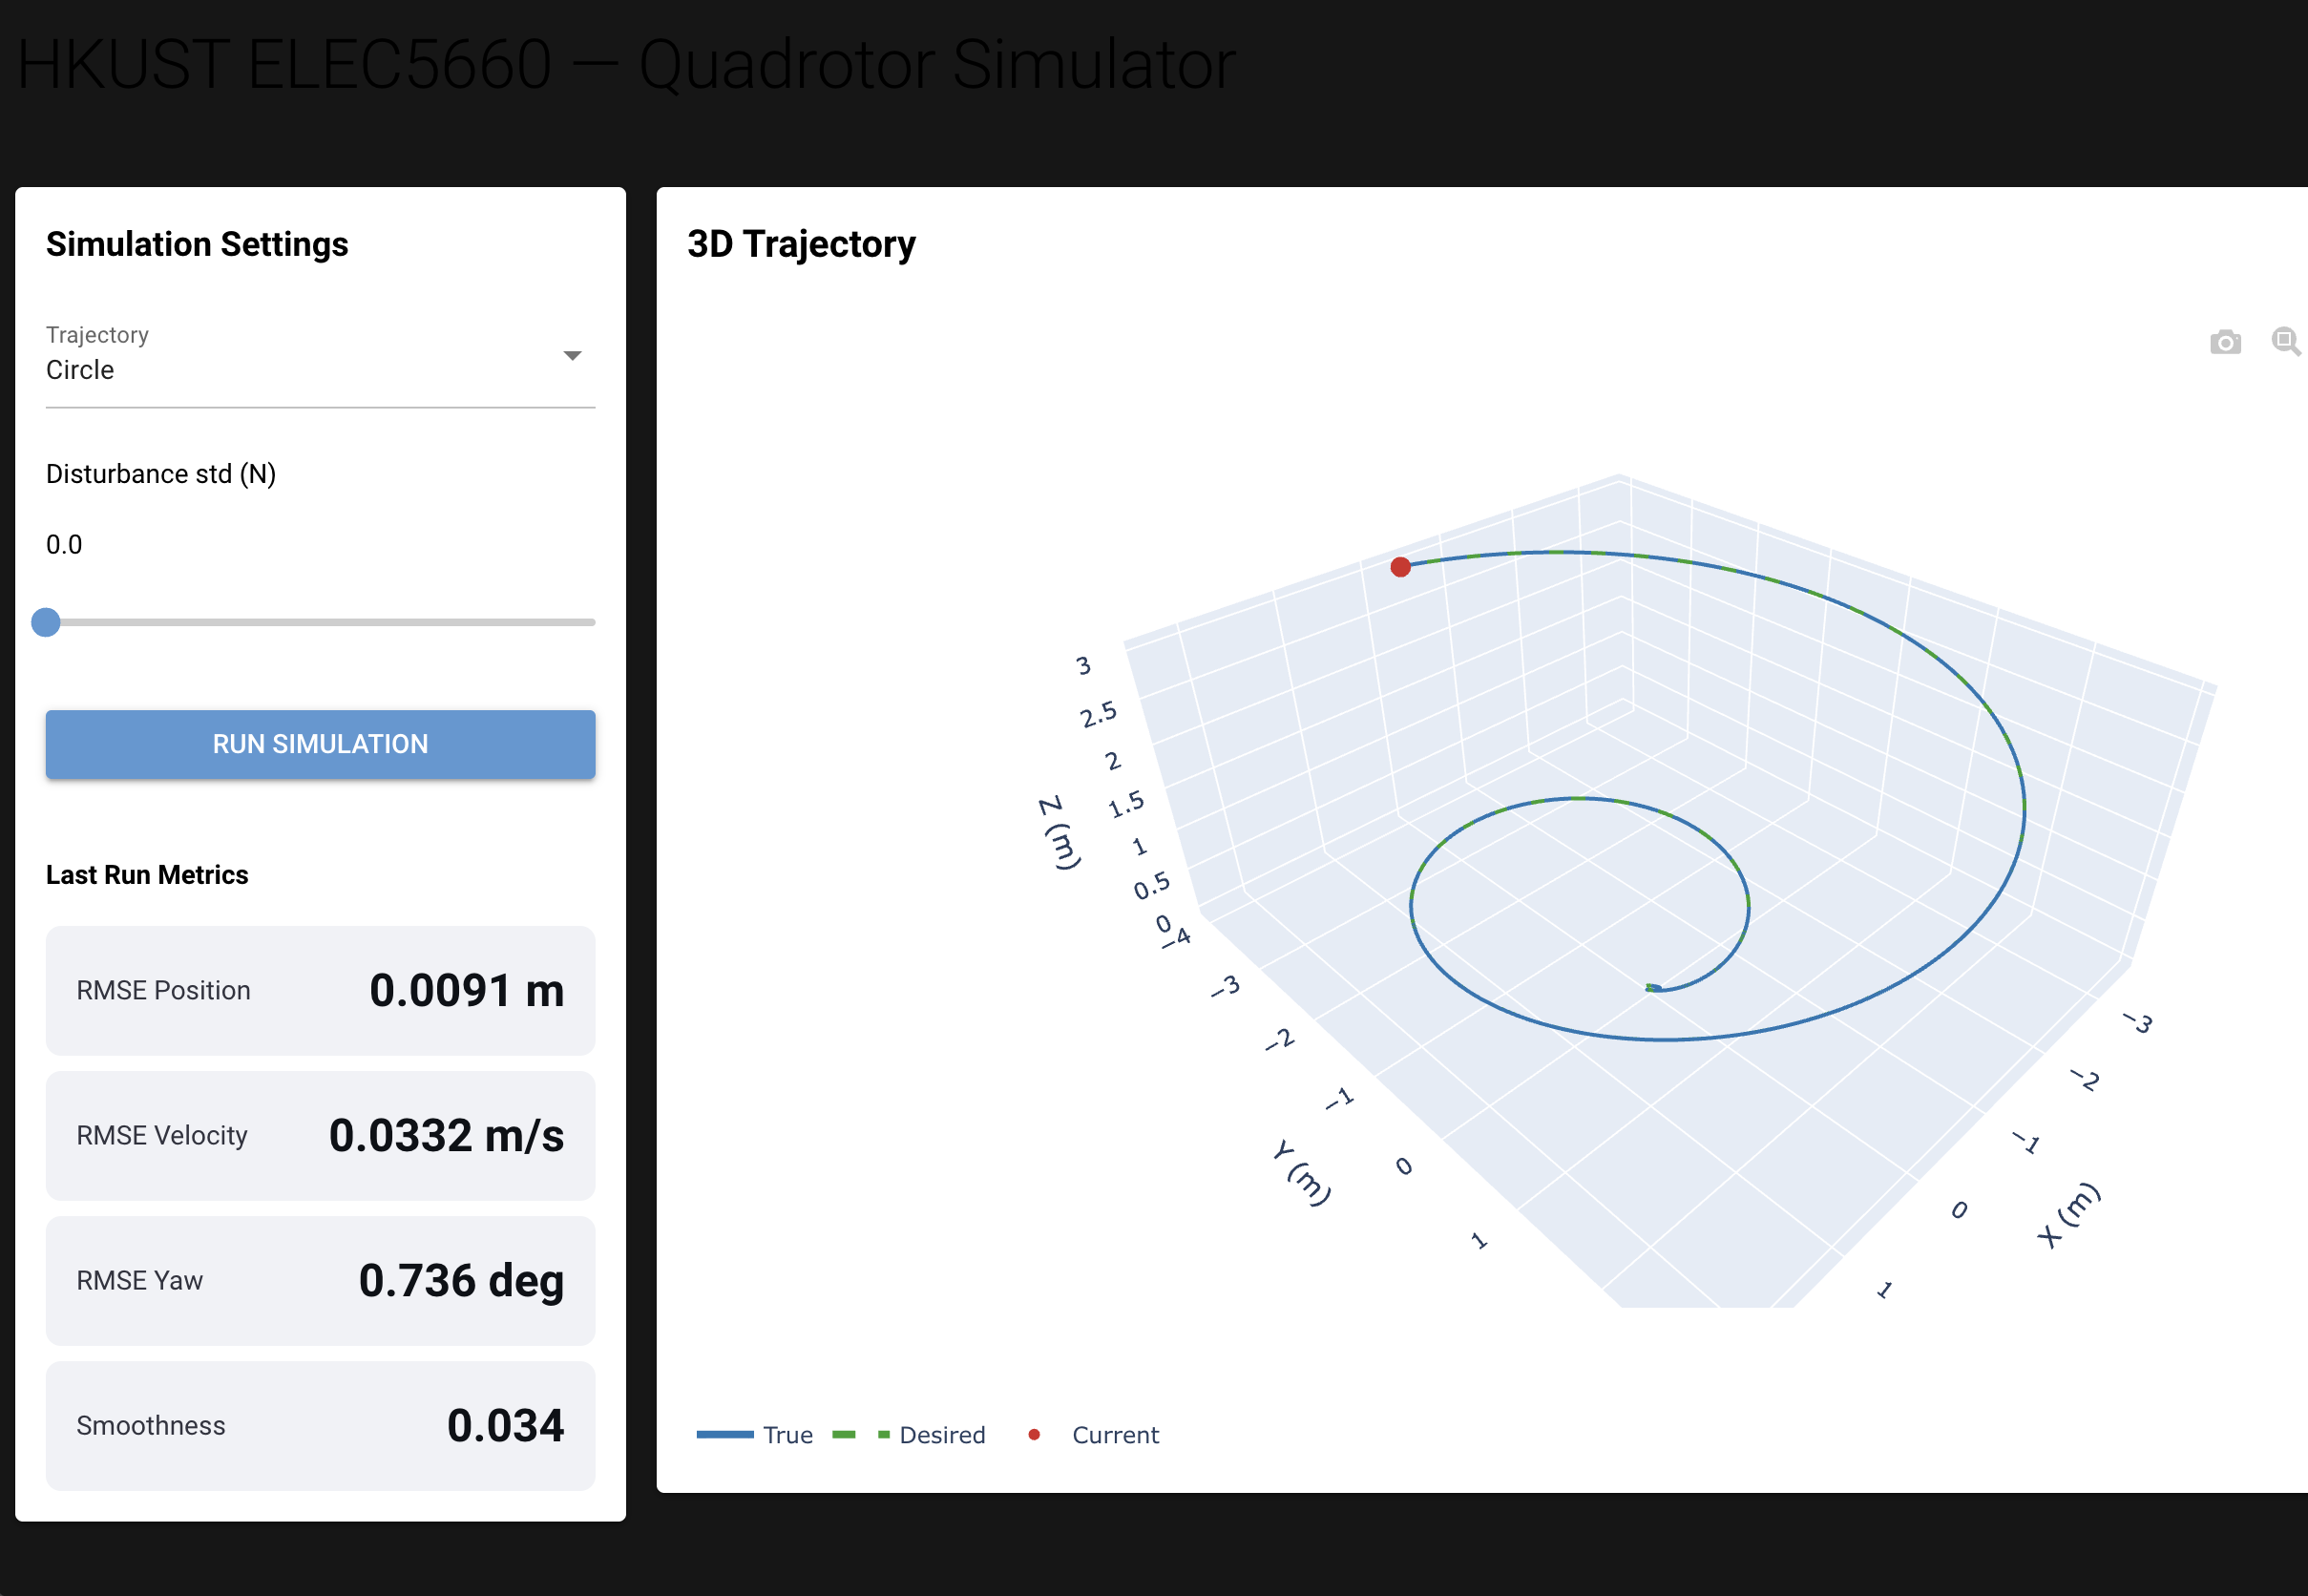
\includegraphics[width=\linewidth]{figs/2.png}
\caption*{circle}
\end{minipage}
\hfill
\begin{minipage}{0.32\linewidth}
\centering
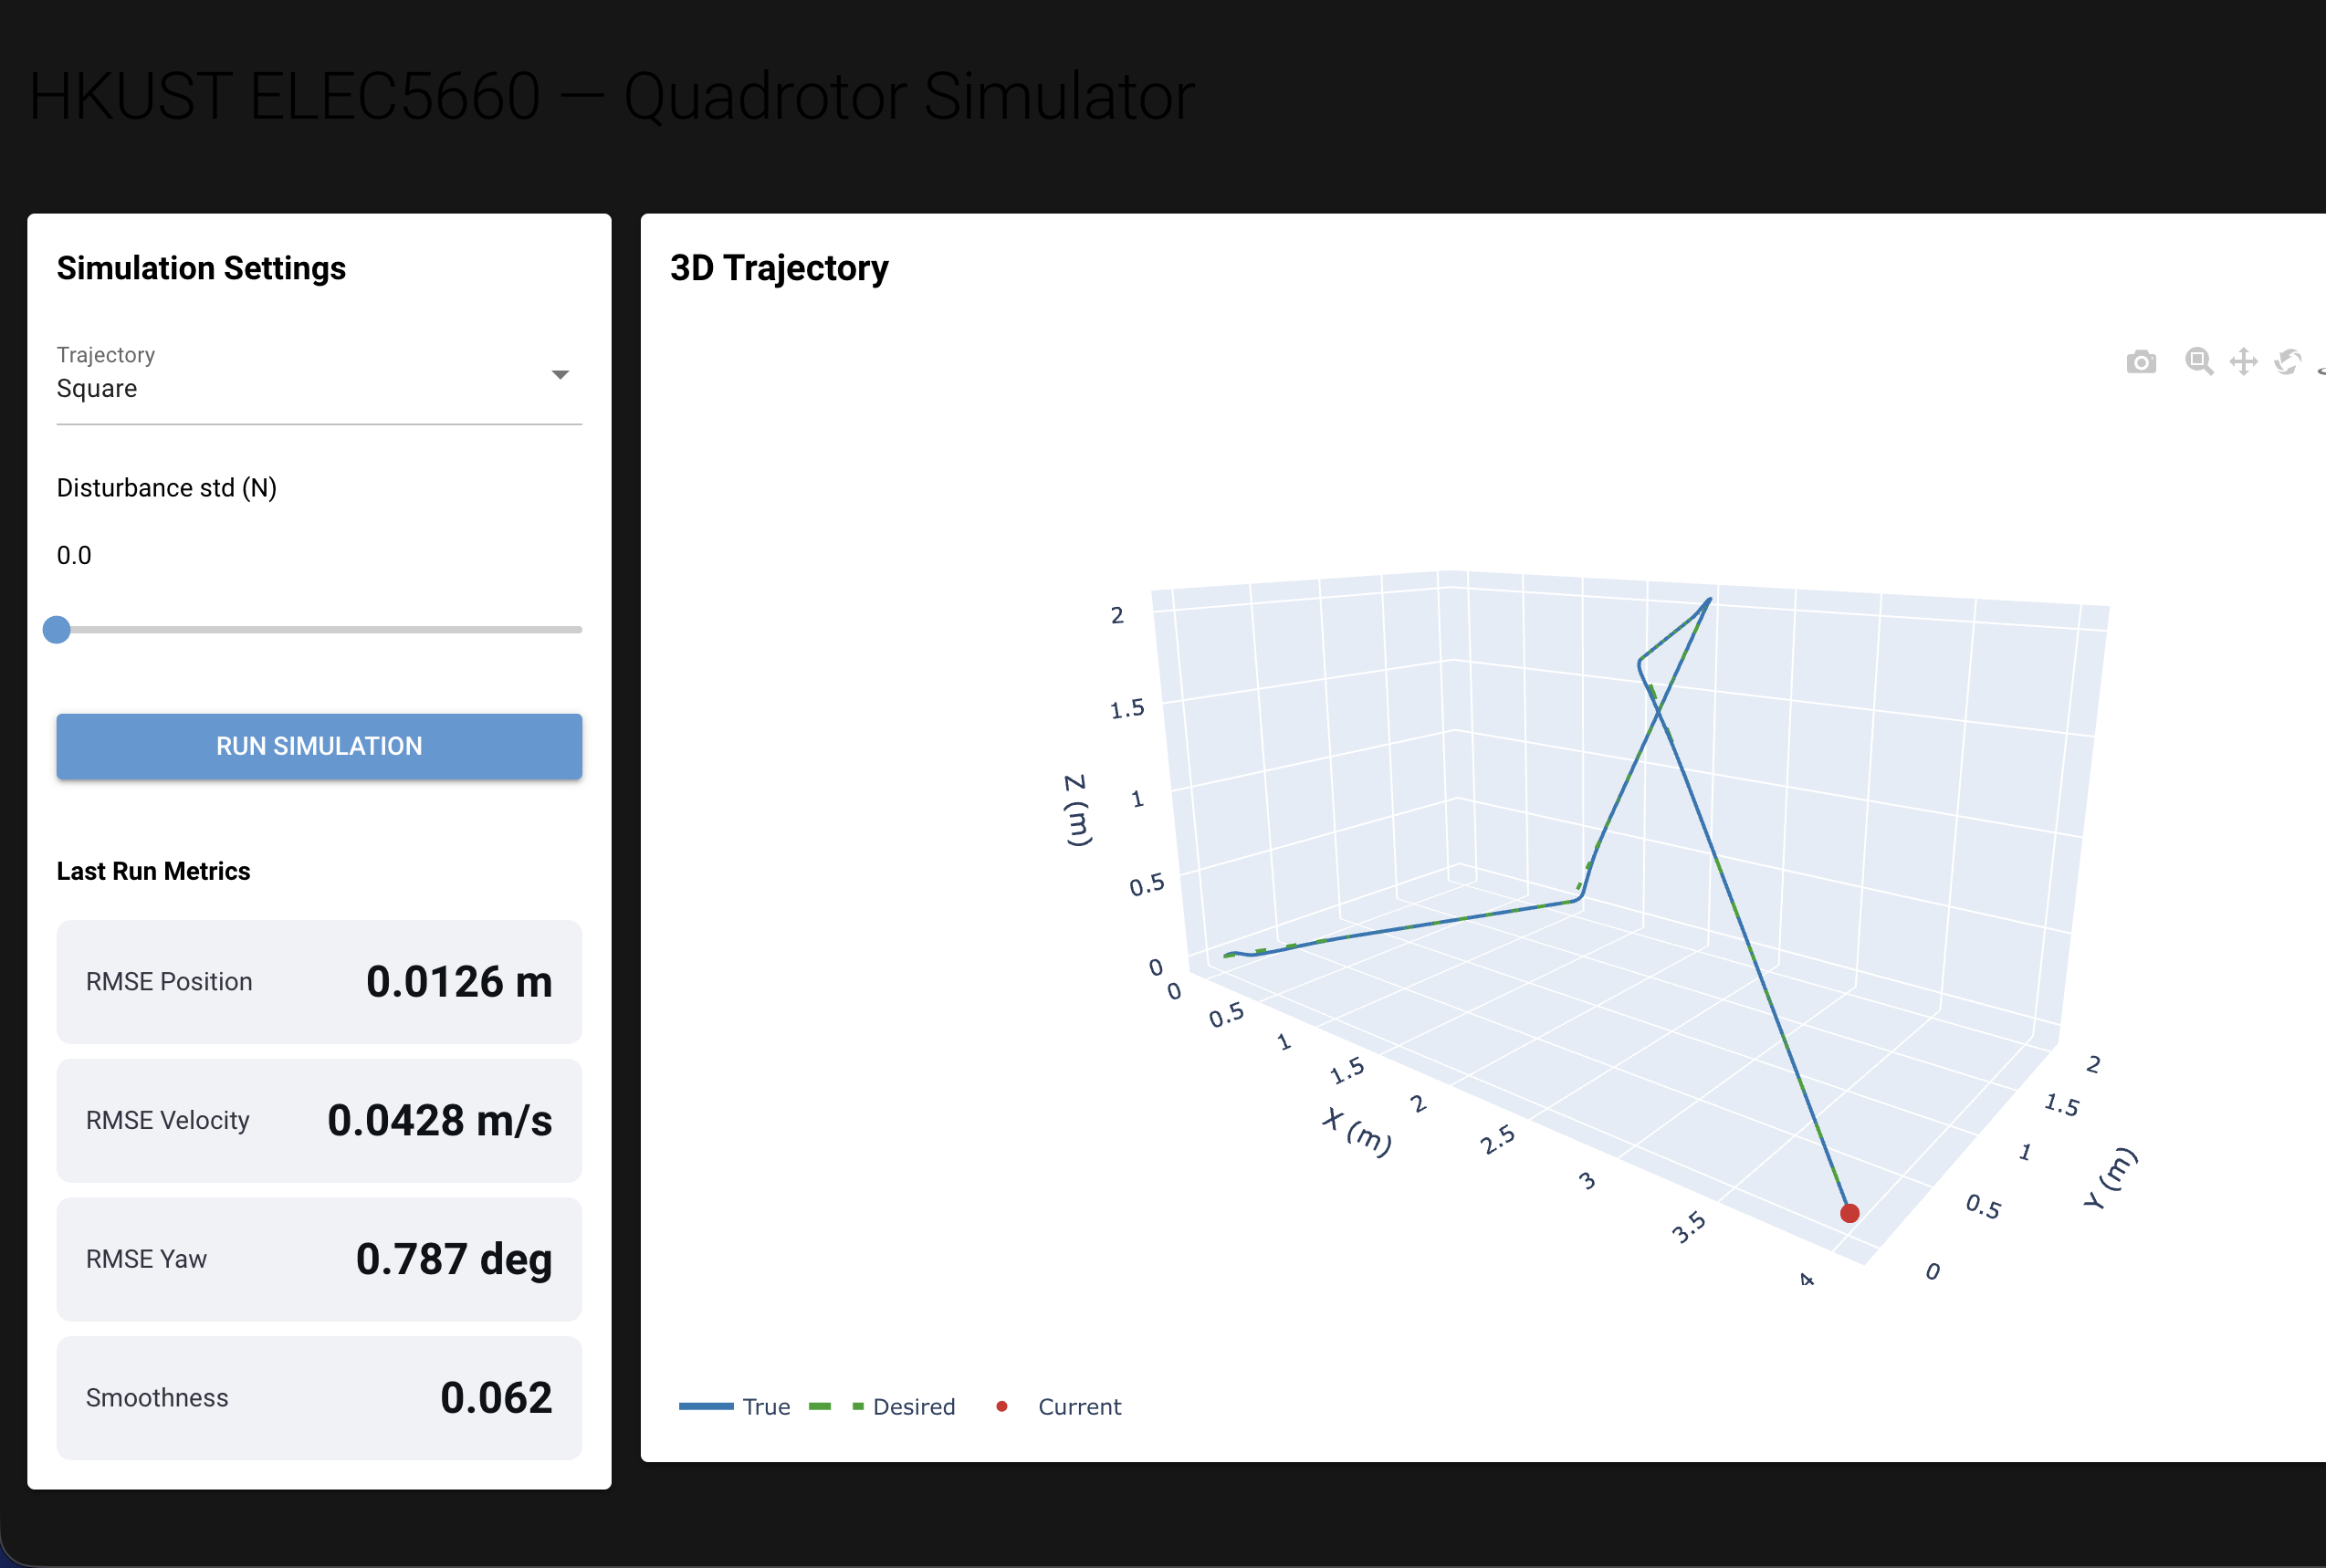
\includegraphics[width=\linewidth]{figs/3.png}
\caption*{square}
\end{minipage}
\hfill
\begin{minipage}{0.32\linewidth}
\centering
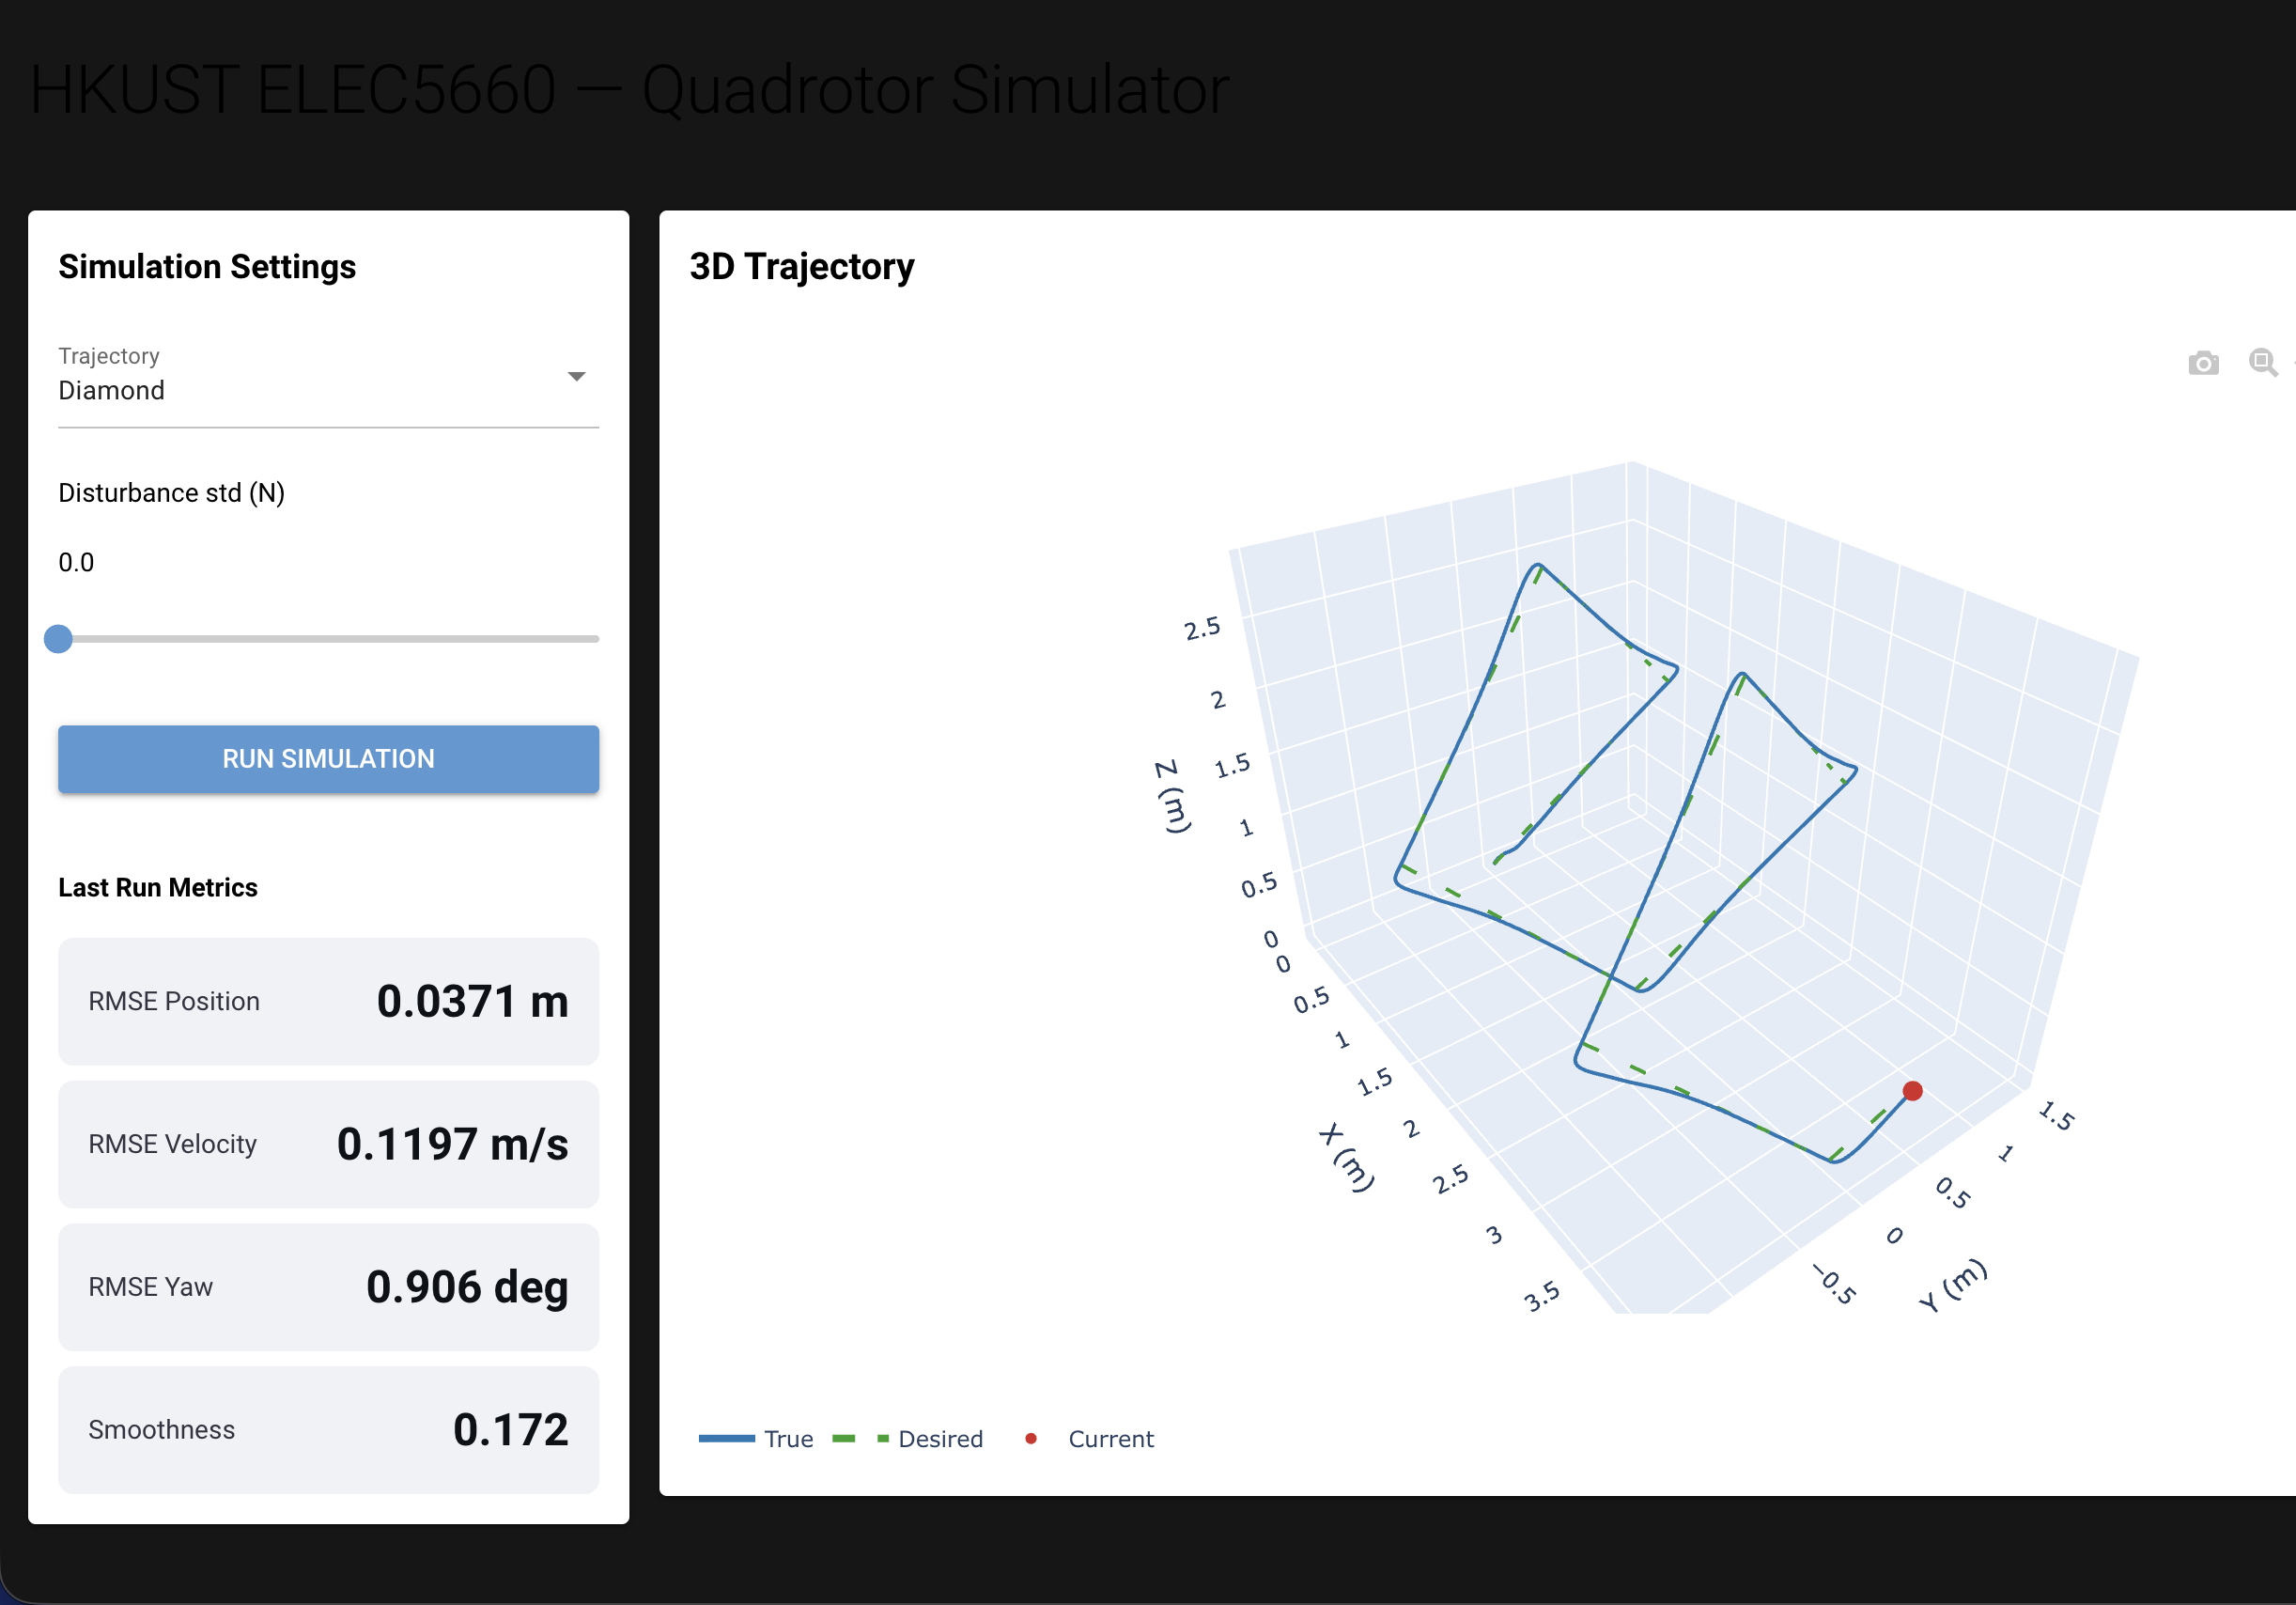
\includegraphics[width=\linewidth]{figs/4.png}
\caption*{diamond}
\end{minipage}
\hfill
\begin{minipage}{0.32\linewidth}
\centering
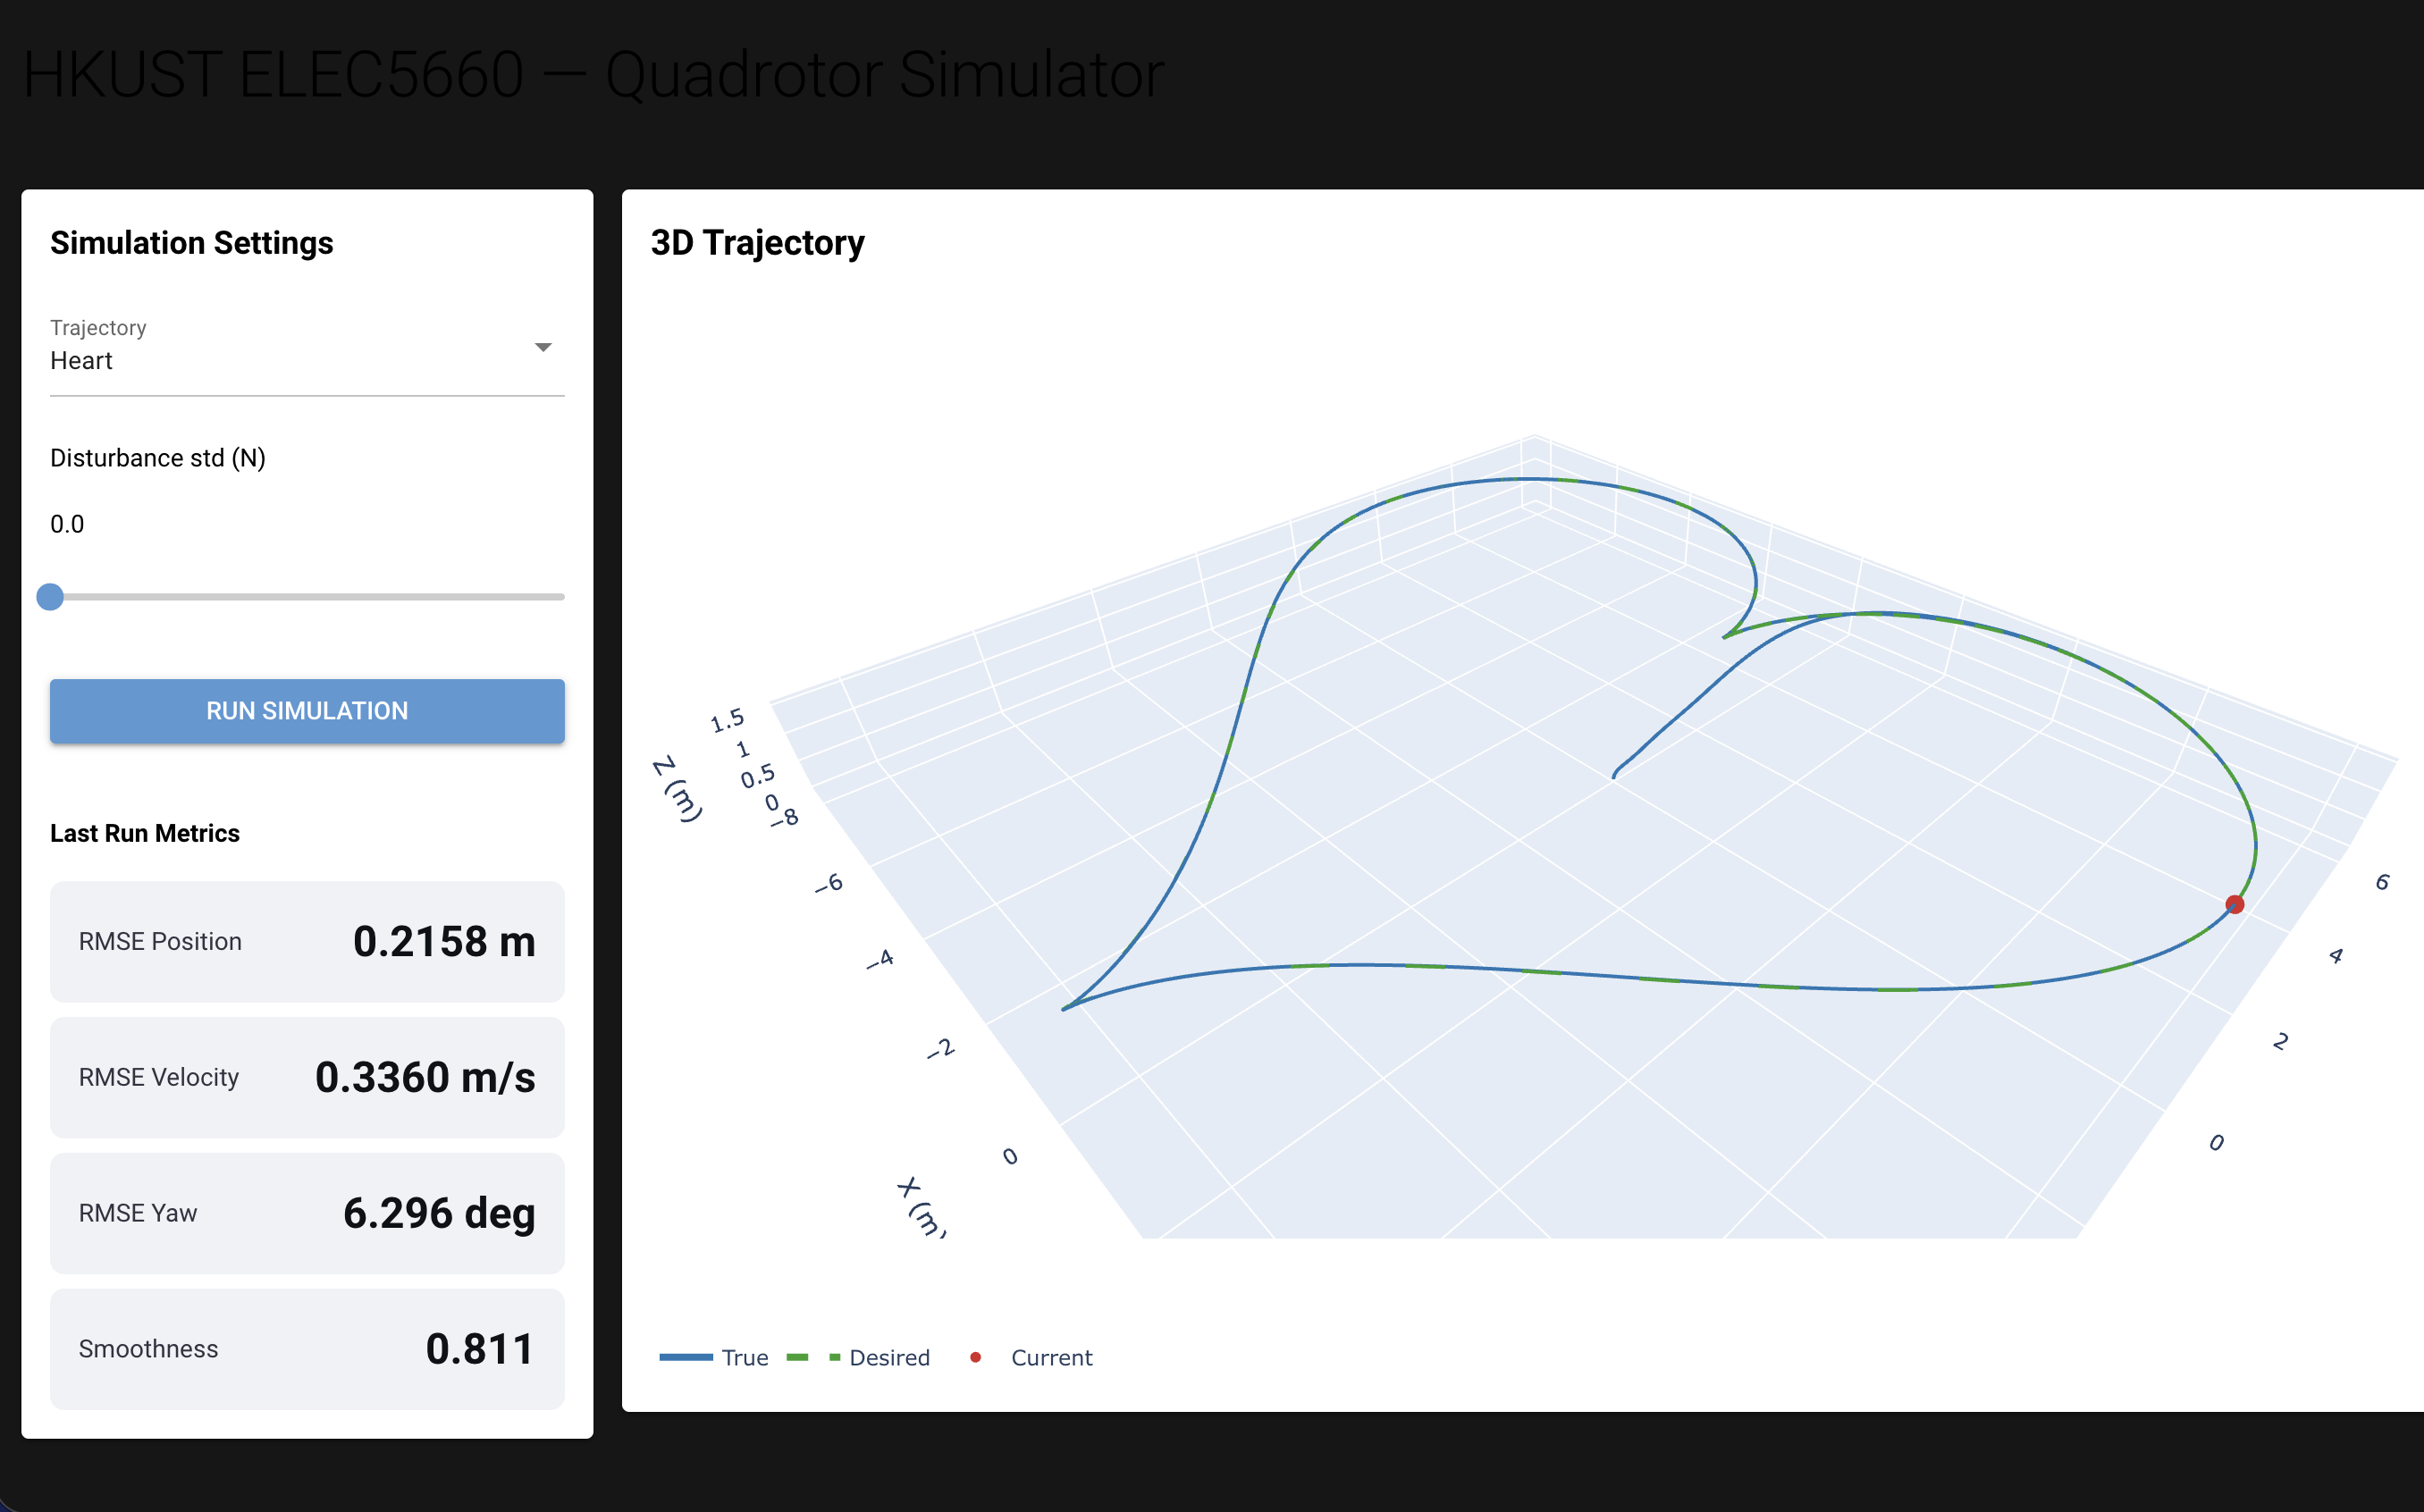
\includegraphics[width=\linewidth]{figs/5.png}
\caption*{heart}
\end{minipage}
\caption{Tracking plots on Path 1,2,3.}
\end{figure}


From the figure1 shows that my pid params can recover the disturbance rapidly.

\section{refernece}
Lecture notes 3 Page 46

\end{document}
